\documentclass[11pt]{article}

%\usepackage[top=2in, bottom=1.5in, left=1in, right=1in]{geometry}
\usepackage{geometry}
\usepackage{amssymb}
\usepackage{algorithm}
% \usepackage{algpseudocode}
\usepackage{amsmath}

\begin{document}

\section{Introduction}
This work explores optimal mesh representation of surfaces using 
triangular surface meshes.
Most mesh generation algorithms refine an initial discretization based
on {\it a priori} error estimates or quality metrics. For example, the
advancing-front algorithm advances boundaries into space to generate a
mesh \cite{tristrano98,diaz-morcillo98}. Other methods generate
meshes from iterative refinement or enrichment from initial, coarse
configurations \cite{marcum98,marcum00,shewchuk02}. These mesh
generation strategies focus on element quality---with the
justification being that downstream applications require high quality
geometries in order to achieve a desired level of accuracy. These
approaches, both historically and in a modern sense, have been 
spectacularly successful at producing high quality meshes for 
computational simulation.

Traditionally, surface mesh generation processes produce good quality
meshes from the combination of geometric growth rates and smoothing.
However, the process requires input, and if the input, or starting place,
is not appropriate, then the geometry is often under and/or oversampled
for the intended use. That fact is not an indictment of the mesh
generation process, but instead implies that the final mesh is heavily
dependent on the inputs. In addition, if some way of controlling the
node spacing in the middle of the surface (away from the boundaries) is
not present, then more nodes could be wasted/omitted in an attempt to
accurately represent the geometry. Efforts have gone into
creating a locally or globally optimal surface mesh. For example,
curvature is a common driver of surface mesh adaptation or refinement
\cite{siqueria13}. Interpolation error, given a desired function, 
is also ubiquitous \cite{peraire87,alauzet06,buscaglia97,huang05}.

The work presented here is contrasted with the above work in that only
the degree in which the discretization approximates the geometry is
considered.  Here formal definitions of fundamental mesh operations
(triangle split, edge split, edge collapse, and vertex movement) are
developed with respect to a locally optimal representation via 
triangular surface meshes for a continuous, parameterized surface. The 
proposed algorithm is a general-use method
that can be applied to any three-dimensional surface regardless of its 
representation.
This is due to every step being developed without the use of
derivatives. A result of not using derivatives is that each step in the
algorithm is robust to large or discontinuous changes in derivatives.

This process can only be automated if some way of judging ``how well'' a
surface mesh represents a surface is present. To this end, a method of
generating surface meshes through constrained, local optimization is
detailed below. Results for mesh representation and efficiency are also
given and discussed.  Further discussion of robustness and mesh quality
is also presented.

Element quality is not considered here as a constraint or goal of the 
optimization procedure, as there
are numerous methods for surface mesh quality optimization
\cite{frey1998,garimella2002,garimella2004a,garimella2004b,jiao2005,jiao2006,jiao2011,jiao2013,lopez2008,montenegro2005,montenegro2006,montenegro2008,montenegro2011,roca2012,roca2013,shivanna2010,zhang2009}
which could be used in a postprocessing step if greater mesh quality is
required.  Instead only optimal representation of the underlying
geometry via triangular surface meshes is studied.


\section{Related Work}

\section{Discretization Error, Discrete Curvature Approximation}
[TALK HERE ABOUT HOW AN OSCULATING ELLIPSOID COULD BE FORMED BY CONSIDERING THE PRINCIPAL CURVATURES AT A POINT BUT THIS REQUIRES DERIVATIVES. ADDITIONALLY, FOR A TRIANGLE AND A GIVEN CANDIDATE POINT, THERE IS NOT ENOUGH INFORMATION TO DEFINE AN ELLIPSOID--ONLY A SPHERE. THEREFORE SOME ANALYSIS WITH AN OSCULATING SPHERE WOULD BE INSTRUCTIVE HERE]

\section{Nomenclature and Definitions}
\subsection{Parametric Surface}
I need a parametric surface so that I can maintain a valid topology.
Projection is not required since the topology gives me uv bounds. The
mesh generation is going on in parametric space. There is an
optimization function for creating the mesh in parametric space. Parametric
space is also great for optimization since you can write the topology
and optimization function constraints in uv space. Mapping a
discretization to a surface in general involved the determination of
"what" an edge means on the surface---whether it's a geodesic line, or
what... If you can do this that's great but the development of a map
is not the purpose of this work so, for ease of presentation, a
parametric surface is used.

Consider an orientable, parameterized surface, $\vec{S}\left(u,v\right)
: {\mathbb R}^2 \rightarrow {\mathbb R}^3$.

\subsection{Discretization}
Consider a discretization, $D$, defined on $S$, comprised of $n_t$
points, $P_i \in \left\{p_1,...,p_{n_t} \right\}$, and a
non-overlapping, non-degenerate, consistently oriented, triangular
connectivity $T$. Each triangle in $T$, $t_i$, is defined by points
$\left(p_j, p_k, p_m\right)$, and edges $\left(e_n, e_o,
e_p\right)$---where the edges are defined (for $t_i$) as $e_n
\left(p_j, p_k\right)$, $e_o \left(p_k, p_m\right)$, $e_p \left(p_m,
p_j\right)$. For the purposes of defining an edge in this work, the
ordering of the nodes does not matter. However, the ordering is used to
maintain consistent orientation during topological operations and to
define constraints in the developed optimization strategy.

Each point, $p_i$, in $D$ is defined at a $\left(u,v\right)_i$
coordinate, and edge is a straight line in both parametric space and in
${\mathbb R}^3$. This is not the case for a discretization which is
mapped onto a surface. In the absence of a parameterization the mapping
of an edge in ${\mathbb R}^3$ to a curve (possibly a straight line, but
    not guaranteed) on a surface is an ambiguous task which is outside
the scope of this work. Additionally, the development of topological
constraints for optimization, which will be detailed later, would not be
as straightforward as is possible when using a parameterized, planar
space.[MAYBE MORE ON THIS AND MAYBE MOVE THIS TO ANOTHER SECTION OR
REORDER TOPICS]

\subsubsection{Toplogy}
By ordering each the connectivity for each triangle in $T$ such that it
has a positive normal, it is straightforward to maintain valid
(non-overlapping) topology during optimization. This is done by not
allowing a topological change, such as an edge swap or nodal movement,
that creates invalid topology.

\subsection{Representation Deficit}
The concept of representation deficit was discussed [REFERENCE] in the
context of curve discretizations. Here, the concept will be extended to
two dimensions. Representation deficit is defined for an operation:

[SCALE INDEPENDENCE]

\subsubsection{Triangle}
A triangle is a planar object, and is representing a possibly non-planar
portion of a surface. Any triangle, with area $A_T$, in the
discretization can have at most the same area as the portion of the
surface which it represents, $A_S$. Therefore, the representation
deficit for a triangle, $RD_T$, can be defined as $RD_T = \frac{A_S -
A_T}{A_T}$. Note that the areas are calculated in ${\mathbb R}^3$. The
difference in surface area, $\left(A_S - A_T\right)$, is normalized by
$A_T$ so that the result is scale independent. Also, this is a
representation {\it deficit} since $A_S \ge A_T$ is always true.

In order to apply the above definition of representation deficit to a
mesh generation, a replacement for $A_S$ must be determined since the
area of the surface represented by $A_S$ is not always able to be
determined --- or, most often, the area calculation is impractical.
Generally, in order to reduce the representation deficit for a triangle
the triangle is split by inserting an interior point. Any point that is
inserted into the interior of the triangle would decrease the
representation deficit --- or at worst it will remain the same. However,
the determination of where to split the triangle should be done in such
a way that the representation deficit is minimized. This strategy of
refinement, refining each triangle in such a way that the representation
deficit is locally minimized,  would take advantage of the optimal
substructure the discrete topology.

The process of determining where to split a triangle is defined here by
a locally optimizing an objective function defined for a triangle: Let
$S(u,v)$ be a parameterized surface, $D$ be be a discretization of the
surface, and $T$ be a triangle (included in $D$) defined by an ordered
tuple of nodes, $\left(n_i, n_j, n_k\right)$. These nodes are ordered
such that the triangle normal is positive. Specifically, if $\vec{V_0} =
\left\{n_j - n_i \right\}$ and $\vec{V_1} = \left\{n_k - n_i\right\}$
then the triangle normal, $N_T = \vec{V_0} \times \vec{V_1}$, is
positive. Note that a two-dimensional cross-product (or two-dimensional
curl) is a scalar quantity. Additionally, let a node on the interior of
$T$ be defined as $n_O$. The four nodes, $n_i, n_j, n_k, and n_O$ define
three triangles, $T_i\left(n_i,n_j,n_0\right), T_j\left(n_j, n_k,
n_0\right), T_k\left(n_k, n_i, n_0\right)$. If $A(T)$ is a function that
calculates the area of a triangle in $\left(x,y,z\right)$ space, then
the optimization problem for finding the optimal position for $n_0$ in
$T$ can be stated as:

\begin{eqnarray*}
\begin{array}{rcl}
\underset{n_O}{\text{minimize}} \ O(T) & = & -\left(A\left(T_i\right) + A\left(T_j\right) + A\left(T_k\right) \right) \\
\text{subject to} \ N_{T_i} & > & 0 \\
N_{T_j} & > & 0 \\ 
N_{T_k} & > & 0 \\
\end{array}
\end{eqnarray*}

\subsubsection{Edge}
An edge in parametric space represents a (possible) curve on the
surface. Any edge, with length $L_E$, can have at most the same length
as the portion of the surface which it represents, $L_S$. Therefore, the
representation deficit for an edge, $RD_E$, can be defined as $RD_E =
\frac{L_S - L_E}{L_E}$. Note that the lengths are calculated in
${\mathbb R}^3$. The difference in length, $\left(L_S - L_E\right)$, is
normalized by $L_E$ so that the result is scale independent. Also, this
is a representation {\it deficit} since $L_S \ge L_E$ is always true;

In order to apply the above definition of representation deficit to mesh
generation, a replacement for $L_S$ must be determined since the area of
the surface represented by $L_S$ is not always able to be determined --
or, most often, the arc-length calculation is impractical.
Generally, in order to reduce the representation deficit for an edge 
the edge is split by inserting an interior point. Any point that is
inserted into the interior of the edge would decrease the
representation deficit --- or at worst it will remain the same. However,
the determination of where to split the edge should be done in such
a way that the representation deficit is minimized. This strategy of
refinement, refining each edge in such a way that the representation
deficit is locally minimized,  would take advantage of the optimal
substructure the discrete topology. A method for generating a locally
optimal edge split is detailed in [REFERENCE SELF].

In addition, the fact that and edge split will change the surface area
of the discretization should be considered. Since the overall
justification of this work is reduce the {\it area} representation
deficit of a discretization, the representation deficit will not be
defined for an edge but for an edge-split. Therefore, for a given edge,
only the edge-split that minimizes representation deficit is considered.
. The process of determining where to split a triangle is defined here
by locally optimizing an objective function defined for an edge-split.
Let $E\left(n_i,n_j\right)$ be an edge in $D$ that is shared
topologically by two triangles, $T_i\left(n_i,n_j,n_k\right)$, and
$T_j\left(n_i,n_l,n_j\right)$. Additionally, let a node on the interior
of the edge be defined as $n_O$. The five nodes, $n_i,n_j,n_k,n_l,n_O$
define four triangles, $T_a\left(n_i,n_O,n_k\right), T_b\left(n_O,n_j,
n_k\right), T_c\left(n_i,n_l,n_O\right), T_d\left(n_O,n_l,n_j\right)$.
The optimization problem for finding the optimal position for $n_O$ on
$E$ can be stated as:

\begin{eqnarray*}
\begin{array}{rcl}
\underset{n_O}{\text{minimize}} \ O(E) & = & -\left(A\left(T_a\right) + A\left(T_b\right) + A\left(T_c\right) A\left(T_d\right) \right) \\
\text{subject to} \ N_{T_a} & > & 0 \\
N_{T_b} & > & 0 \\ 
N_{T_c} & > & 0 \\
N_{T_d} & > & 0 \\
\end{array}
\end{eqnarray*}

\subsubsection{Edge Flipping}
Is it possible to have an optimal topology? If so, then it should be
reachable through repeated edge flipping. Therefore, we should be able
to write some sort of formulation for a pair of triangles and go from
there? [SUZANNE] Comment: for the sake of not doing any more coding, if
your ethics can let you come to the conclusion that this is either not
possible or not practical then this would fit into the
logic/justification in the next section.

\subsubsection{Nodal Smoothing}
For a node, $N_i$, the representation deficit can be defined only by
comparing it to the node when located at another point in space. Here
the comparison is bound by limiting the range of comparison within the
edge-hull topologically adjacent to $N_i$. Formally, let $N_i$ be a node
in $D$ that is shared topologically by $n$ triangles, where $n$ is the
face-valence of $N_i$. The optimization for finding the optimal position
for $N_i$ can be stated as:

\begin{eqnarray*}
\begin{array}{rcl}
\underset{N_O}{\text{minimize}} \ O(N) & = &
-\sum{_{j=1}^{n_t-1}A\left(T_j\right)} \\
\text{subject to} \ N_{T_1} & > & 0 \\
N_{T_2} & > & 0 \\ 
N_{T_3} & > & 0 \\
& \vdots & \\
N_{T_{n-1}} & > & 0 \\ 
N_{T_n} & > & 0
\end{array}
\end{eqnarray*}


\section{Optimal Substructure vs Global Optimization}
In order to formulate an optimization problem which, when solved, yields 
an optimal mesh triangulation based on representation deficit, a local 
optimization approach~\cite{nocedal_wright_book} is used. Such a 
formulation comes much more naturally than does a formulation based on 
global optimization~\cite{global_optimization_book} when the 
mesh operations defined in Section \ref{sec:meshoperations} are 
employed. One reason for this is the variety of mesh operations that are 
performed at different stages in the mesh generation process; they 
naturally lend themselves to the formulation of different (but related) 
optimization problems as opposed to one unified optimization problem.

It should also be noted that global optimization algorithms are typically 
not used to solve optimization problems with a large number of variables 
-- even if the problem is formulated as a global optimization problem. 
Since there are typically millions to billions of nodes and elements in 
meshes from application problems of interest, a global optimization 
problem would be impractical solve based on the huge number of variables 
that it would necessarily contain. In addition, any global optimization 
problem which would be formulated as a generalization of the local 
optimization problems in this work would be a continuous optimization 
problem. Typically global optimization methods are designed for use on 
discrete optimization problems or on contious optimization problems with 
convex objective functions with guaranteed global minima.

For the above reasons, iterative refinement (a local optimization 
approach) is used to find optimal substructures at each stage of the mesh 
generation process. The local optimization technique employed is
motivated by a class of optimization methods called pattern search 
techniques~\cite{patternsearch1}. Pattern search and multidirectional 
search techniques were developed by Park and Shontz for mesh quality 
improvement~\cite{patternsearch4}; their techniques were based on the 
underlying classes of optimization methods in the literature. Pattern 
search methods do not use derivatives and hence can be used on problems for 
the most general problems for which derivatives either do not exist or are 
impractical to compute.

The optimization employed here uses a simple ``cross'' pattern (up down
left right center, \cite{crossPattern}) {\bf{Dave:  No reference by
with this label appears in the References currently.  Please 
update}} which 
is sized based on the
local geometry so that it could be moved inside of the triangles/hulls
many times before encountering the boundary. In the case of triangle
splitting, the cross was sized as $0.001$ multiplied by the average edge
length of the triangle. In the case of node movement, the cross was
sized as $0.001$ multiplied by the average edge length of the
topologically attached edges. The cross pattern was not resized during
optimization.  Additionally, the search was not allowed to create
inverted elements.  This was enforced by halting a search whose next
step would create any overlapping edges, tangled elements, etc... Care
was taken to ensure that convergence of the local optimization method
was obtained; this is important since criteria must be met in order for
the heuristic pattern search methods to
converge~\cite{patternsearch2,patternsearch3}.

\begin{figure}
  \begin{center}
  \label{crossPattern}
  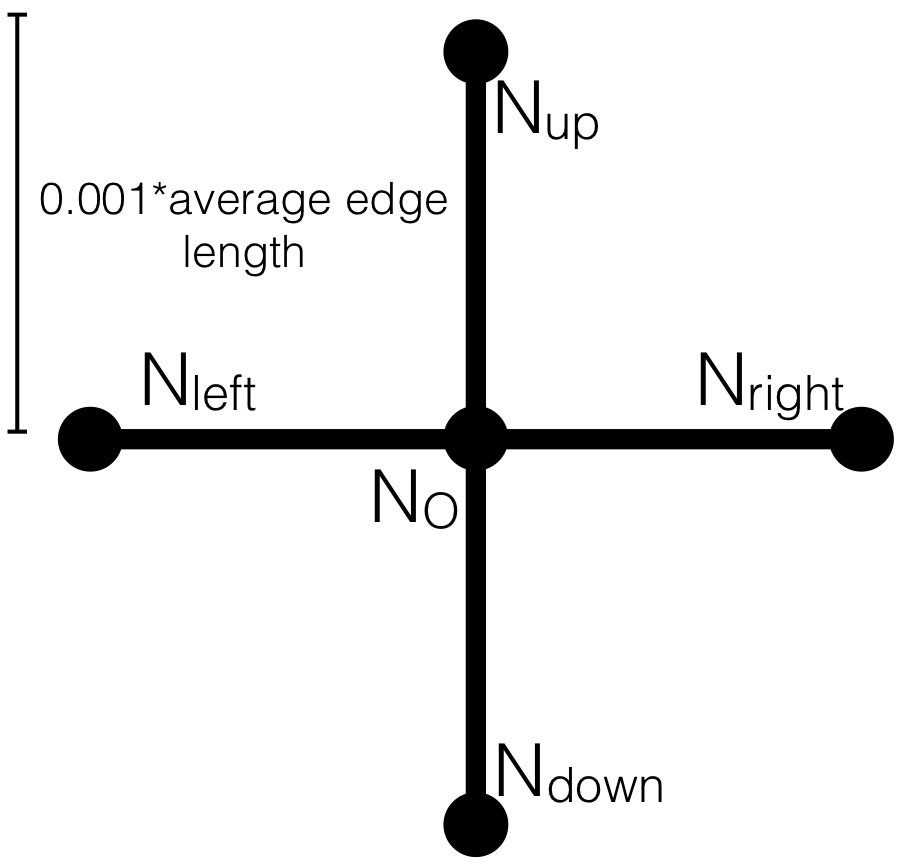
\includegraphics[width=50mm]{Figures/crossPattern.png}
  \caption{Cross Pattern used for Pattern Search Optimization}
  \end{center}
\end{figure}


\section{Element Quality}
[SHOULD THIS EVEN BE A SECTION. IT NEEDS TO BE DISCUSSED BUT I'M NOT
SURE THAT IT NEEDS IT'S OWN SECTION

\section{Results}

\section{Conclusions}

\section{Acknowledgements}

\bibliographystyle{amsplain}
\bibliography{References}
\end{document}
